\documentclass[11pt]{article}

% ---------- packages ----------
\usepackage[margin=1in]{geometry}
\usepackage{graphicx}
\usepackage[T1]{fontenc}
\usepackage{lmodern}
\usepackage{microtype}
\usepackage{amsmath,amssymb}
\usepackage{xcolor}
\usepackage{booktabs}
\usepackage{array}
\usepackage[font=small,labelfont=bf,labelsep=period]{caption}
\usepackage{authblk}
\usepackage[numbers,sort&compress]{natbib}
\usepackage{enumitem}
\usepackage[colorlinks=true,allcolors=blue!55!black]{hyperref}
\usepackage{titlesec}

\titleformat{\section}{\large\bfseries\sffamily}{\thesection}{0.6em}{}
\titleformat{\subsection}{\normalsize\bfseries\sffamily}{\thesubsection}{0.6em}{}
\renewcommand{\abstractname}{\sffamily\bfseries Abstract}

% ---------- macros ----------
\newcommand{\zlin}{\ensuremath{z_{\mathrm{lin}}}}
\newcommand{\ziv}{\ensuremath{z_{\mathrm{iv}}}}
\newcommand{\tauH}{\ensuremath{\tau_{H}}}
\newcommand{\tauR}{\ensuremath{\tau_{R}}}
\newcommand{\nref}{2{,}615{,}898}
\newcommand{\nquery}{1{,}767{,}346}

\title{\sffamily\bfseries NullState: a reference-anchored framework for detecting,\\ diagnosing, and quantifying the off-target compartment of\\ human neural organoids}

\author[1]{Luiz T.\ Takahashi}
\affil[1]{\normalsize\itshape Independent research; correspondence: \texttt{ltaktakahashi@gmail.com}}
\date{\today}

\begin{document}
\maketitle

\begin{abstract}
\noindent Human neural organoids reproducibly generate cell types that lie outside the developmental
trajectories they are intended to model, but the field lacks a principled, atlas-anchored way to
\emph{quantify} this off-target compartment and ask whether it carries reproducible structure.
We present \textbf{NullState}, a reference-based pipeline that maps the \nquery-cell Human Neural
Organoid Atlas (HNOCA) onto a harmonized \nref-cell first-trimester human fetal reference
(HDBCA $+$ a fetal-body atlas) by variational reference surgery, assigns each organoid cell a pair of
calibrated mapping scores (off-manifold distance and label entropy), and classifies it into a
six-state off-target taxonomy. Across the atlas, $38.4\%$ of cells fall into an
\emph{ambiguous-novel} (off-manifold) compartment. Four orthogonal diagnostics show this compartment
is not a projection artifact but a \emph{structured mixture} of a reference-coverage gap and a
pervasive in-vitro stress program: off-manifold cells lose neural-progenitor identity while gaining
hypoxia and unfolded-protein-response signatures, their burden rises monotonically with maturation and
metabolic load, varies $\sim$240-fold across differentiation protocols ($0.4\%$ to $96.8\%$), and
concentrates into coherent transcriptomic clusters. We then show, as a reproducible \emph{negative}
result, that a shared-latent contrastive generative model cannot separate lineage from in-vitro state
here: an origin-decoding adversary recovers organoid-versus-primary identity from the putatively
dish-stripped latent at $\geq\!0.998$ balanced accuracy, robustly across latent-capacity and
batch-conditioning interventions, because the in-vitro state is transcriptome-pervasive rather than a
separable nuisance subspace. Finally, we demonstrate that off-target geometry is nonetheless
recoverable: among well-powered off-target populations, all pairwise lineage distances are real
(clearing a matched-$N$ noise floor by $14$--$105\times$) and biologically ordered, with the two
myogenic populations closest in the embedding. NullState provides a deployable off-target quality axis
for organoid studies and a precise account of when latent disentanglement is and is not attainable.
\end{abstract}

\vspace{0.5em}

% =====================================================================
\section{Introduction}
% =====================================================================
Human pluripotent-stem-cell-derived neural organoids have become a central model of human brain
development \citep{lancaster2013organoids,pasca2015cortical}, capturing cortical cytoarchitecture,
diverse neuronal and glial identities, and functional network activity
\citep{quadrato2017organoids,velasco2019organoids,trujillo2019oscillatory}. Yet a recurring concern
limits their interpretation: organoids also produce cells that do not correspond to any \emph{bona
fide} in-vivo neural state. These include non-neural lineages arising from incomplete germ-layer
restriction and aberrant states driven by the culture environment itself. A landmark observation is
that metabolic and endoplasmic-reticulum (ER) stress in organoids impairs the specification of correct
molecular subtypes \citep{bhaduri2020stress}, and cross-protocol comparisons against fetal tissue have
repeatedly surfaced protocol-dependent, off-target differentiation routes
\citep{tanaka2020synthetic,kanton2019atlas}. The recent Human Neural Organoid Atlas
(HNOCA)---an integrated transcriptomic atlas of $>$1.7~million organoid cells spanning dozens of
protocols \citep{he2024hnoca}---makes it possible, for the first time, to study this off-target
compartment at scale and against a common coordinate system.

What has been missing is a \emph{principled, reference-anchored} way to (i) decide which organoid cells
are off-target, (ii) explain \emph{why} they are off-target, and (iii) ask whether the off-target
compartment is merely noise or carries reproducible biological structure. Reference-based mapping
provides the natural substrate: by projecting organoid cells onto a comprehensive fetal atlas, cells
that map confidently to a fetal identity can be separated from those that do not. Two
recently completed human references make such anchoring feasible---a comprehensive first-trimester
human brain cell atlas (HDBCA) \citep{braun2023hdbca} and a human fetal-body gene-expression atlas
\citep{cao2020fetal}---together spanning neural and non-neural developmental origins.

Here we introduce \textbf{NullState}, a pipeline that operationalizes this idea (Fig.~\ref{fig:overview}).
We harmonize the two fetal atlases into a single \nref-cell reference, map the \nquery-cell HNOCA query
onto it by variational reference surgery \citep{lopez2018scvi,xu2021scanvi,lotfollahi2022scarches},
and assign every organoid cell two calibrated mapping scores---an off-manifold reconstruction distance
and a label-assignment entropy---that jointly define a six-state off-target taxonomy. We organize the
analysis around three questions: \textbf{(Aim~1)} is the off-target measurement well-posed and
adequately powered? \textbf{(Aim~2)} can lineage biology be disentangled from the in-vitro state, so
that off-target cells can be placed on a ``dish-stripped'' lineage axis? and \textbf{(Aim~3)} do
off-target populations occupy distinct, reproducible geometry? Our central findings are that the
dominant off-manifold compartment is a structured biological mixture rather than an artifact; that
shared-latent disentanglement provably fails here for an interpretable reason; and that off-target
geometry is nevertheless recoverable and biologically coherent.

% =====================================================================
\section{Results}
% =====================================================================

\subsection{A harmonized fetal reference supports confident organoid mapping}
We assembled a fetal reference by combining the first-trimester HDBCA \citep{braun2023hdbca} with the
non-neural compartments of a human fetal-body atlas \citep{cao2020fetal}, retrieving raw unique-molecular-identifier
(UMI) counts from the CZ~CELLxGENE Discover Census \citep{czi2025cellxgene}. The merged reference
comprises \nref{} cells $\times$ 61{,}497 genes, with $32/33$ lineage origins resolved. We trained a
single-cell variational model (scVI) for 400 epochs (evidence lower bound, ELBO, $695.6$), refined it
into a label-aware model (scANVI, ELBO $736.1$), and projected the HNOCA query onto the reference by
architectural surgery (scArches; query-surgery ELBO $920.2$) \citep{lopez2018scvi,xu2021scanvi,lotfollahi2022scarches,gayoso2022scvitools}.
Surgery required two stabilizers that we found essential at atlas scale: excluding $9{,}229$
non-UMI (full-length read-count) cells whose library sizes destabilize the negative-binomial encoder,
and filtering to cells with $\geq\!50$ counts across highly variable genes ($\nquery\rightarrow1{,}689{,}762$;
$4.4\%$ removed).

Donor-level batch integration improved cross-batch mixing while preserving biological structure:
the integration local inverse Simpson's index (iLISI) rose from $6.10$ (unintegrated principal
components) to $8.10$ after scVI, with only a modest change in the cell-type cLISI ($1.31\rightarrow1.44$)
\citep{korsunsky2019harmony,luecken2022scib} (Fig.~\ref{fig:aim1}c). We calibrated two decision
thresholds on held-out reference cells---a label-entropy threshold $\tauH=0.96$ and an off-manifold
threshold $\tauR=1.93$---and used them to assign each organoid cell to one of six states
(Fig.~\ref{fig:aim1}a,b). The resulting partition is dominated by an \emph{ambiguous-novel}
(off-manifold) compartment ($677{,}783$ cells; $38.4\%$), followed by clean on-target ($459{,}441$;
$26.0\%$), poorly differentiated on-target ($281{,}217$; $15.9\%$), ambiguous ($167{,}838$; $9.5\%$),
true off-target ($93{,}795$; $5.3\%$), and quality-control-dropped cells ($86{,}813$; $4.9\%$).

Three feasibility gates confirmed the measurement is well-posed (Fig.~\ref{fig:aim1}d). The off-target
taxonomy is internally consistent (Gate~A, pass); an in-vitro ``dish-vector'' computed on clean
on-target cells is highly self-consistent (Gate~B, mean cosine $0.855>0.70$), justifying a single
shared in-vitro axis; and the true off-target compartment is adequately powered for downstream geometry
(Gate~C, green; $93{,}795$ cells). NullState thus yields a calibrated, adequately powered off-target
measurement over the entire organoid atlas.

\subsection{The off-manifold compartment is a structured mixture of reference gap and in-vitro stress}
The size of the ambiguous-novel compartment ($38.4\%$) raises an essential question: is it a mapping
artifact, or does it reflect real biology? Four orthogonal diagnostics, computed on the neural subset,
converge on the latter (Fig.~\ref{fig:diag}).

\emph{Identity and stress programs (Fig.~\ref{fig:diag}a).} Relative to clean on-target neural cells,
ambiguous-novel neural cells show markedly reduced neural-progenitor identity (NPC score
$1.11\rightarrow0.61$) while gaining canonical stress signatures: hypoxia
($0.60\rightarrow0.96$) \citep{buffa2010hypoxia} and the unfolded-protein/ER-stress response
($0.12\rightarrow0.56$, a $\sim$5-fold increase). An independent, atlas-precomputed glycolysis hallmark
score is correspondingly elevated ($0.46\rightarrow0.65$). This is the transcriptional signature of
culture stress described by Bhaduri \emph{et al.}\ \citep{bhaduri2020stress}, here resolved at atlas
scale and tied directly to off-manifold status.

\emph{Maturation and metabolic load (Fig.~\ref{fig:diag}b).} The off-manifold fraction rises
monotonically with a per-cell potency/complexity proxy (number of detected genes; quintile fractions
$0.13\rightarrow0.78$) and is highest in the oldest organoids (age quintile fraction $0.62$;
median off-manifold score $1.84\rightarrow2.12$ across age) \citep{gulati2020cytotrace}. Off-target
burden therefore accrues with culture time and metabolic demand, consistent with a stress-driven
mechanism rather than random misassignment.

\emph{Protocol dependence (Fig.~\ref{fig:diag}c).} Across 26 differentiation protocols, the
ambiguous-novel fraction spans nearly the entire range ($0.4\%$ to $96.8\%$; standard deviation
$0.28$). Guided cortical protocols sit at the low end (e.g., DAPT-patterned cortico-motor
\citep{andersen2020corticomotor}, $0.4\%$; \citealp{pasca2015cortical}, $10\%$), whereas
regionally divergent or barrier-forming protocols dominate the high end---choroid-plexus organoids
\citep{pellegrini2020csf} reach $96.8\%$, midbrain-dopaminergic \citep{fiorenzano2021midbrain} and
thalamic \citep{xiang2019thalamic} protocols $85$--$90\%$. The off-manifold signal thus partly tracks
\emph{reference coverage}: the first-trimester, cortex-rich HDBCA under-represents later and
non-cortical neural states, which are then read as off-manifold.

\emph{Cluster coherence (Fig.~\ref{fig:diag}d,e).} Ambiguous-novel cells are not scattered. Across 30
Leiden communities in the atlas embedding \citep{traag2019leiden}, the off-manifold fraction is bimodal
(per-cluster s.d.\ $0.29$ about an overall mean of $0.55$); $20\%$ of cells reside in near-pure
off-manifold clusters ($\geq\!80\%$) and $21\%$ in near-pure clean clusters ($\leq\!20\%$). Off-manifold
status is a coherent population-level property, visible as contiguous territory in the scPoli UMAP
\citep{mcinnes2018umap}.

Together these diagnostics establish that the dominant off-target compartment is a reproducible
biological mixture: a \emph{reference-coverage gap} (non-cortical and later neural states absent from a
first-trimester reference) superimposed on a pervasive \emph{in-vitro stress} program (hypoxia,
unfolded-protein response, glycolysis) that intensifies with maturation.

\subsection{Lineage cannot be disentangled from in-vitro state in a shared latent (a characterized negative)}
If the in-vitro state were a low-dimensional nuisance, one could subtract it and place off-target cells
on a clean lineage axis. We tested this directly with contrastiveVI, which factorizes a background
(shared) latent \zlin{} from a salient latent \ziv{} \citep{weinberger2023contrastivevi}, training the
background on primary fetal cells and the salient on organoid cells, so that \zlin{} should encode
dish-stripped lineage. We evaluated disentanglement with a held-out adversary: a classifier that
attempts to recover organoid-versus-primary origin from \zlin{} (balanced accuracy $0.5$ is ideal;
$<0.6$ would indicate success) (Fig.~\ref{fig:aim2}a).

Disentanglement failed, and did so robustly. The baseline model
($\dim\ziv=10$) yielded adversary balanced accuracy $0.998$; tripling salient capacity ($\dim\ziv=30$)
gave $0.999$; and adding a source batch covariate to the decoder---the textbook remedy for a nuisance
axis confounded with a condition---gave $0.998$. Training converged normally in every case
(Fig.~\ref{fig:aim2}b), so this is not an optimization failure. The mechanism is structural
(Fig.~\ref{fig:aim2}c): because the in-vitro state is transcriptome-pervasive (Fig.~\ref{fig:diag})
and organoid and fetal cells occupy near-disjoint regions of expression space, the background
\emph{encoder} $q(\zlin\!\mid\!x)$ observes and encodes source identity directly; conditioning the
\emph{decoder} on a batch label cannot undo what the encoder has already written into \zlin. We
therefore report, as a precise negative result, that shared-latent contrastive disentanglement is not
attainable in the fetal-versus-organoid regime: the dish signature is not a separable subspace but a
global transcriptional shift. This delimits where ``calibration without anchoring'' can and cannot be
applied and motivates encoder-side or distributional alternatives.

\subsection{Off-target populations occupy distinct, biologically coherent geometry}
The disentanglement failure does not, however, invalidate the geometry of off-target populations
relative to one another. Aim~3 compares off-target \emph{organoid} populations against \emph{each
other}; because all such cells share the same organoid-versus-primary offset in \zlin, that offset is a
constant translation that cancels exactly in pairwise sliced-Wasserstein distances
($W(\mathcal{A}{+}c,\mathcal{B}{+}c)=W(\mathcal{A},\mathcal{B})$) \citep{bonneel2015sliced}. The
contamination shifts all populations together and therefore does not distort their relative structure.

We computed pairwise lineage distances among the true off-target populations, controlling for sample
size by a rarefaction-derived minimum ($N_{\min}=2000$) and a matched-$N$ self-distance noise floor; a
pair is called only if its cross-distance confidence interval clears the floor (Fig.~\ref{fig:aim3}).
Of the $17$ off-target populations, four are well powered (cortical-adrenal $49{,}338$;
skeletal-muscle $30{,}629$; fibroblast $6{,}349$; cardiac-muscle $2{,}534$). All six pairwise
comparisons are real differences, each clearing the noise floor by $14$ to $105\times$
($W$ from $0.32$ to $0.99$ against floors of $0.007$--$0.026$); the remaining $130$ small-$N$
comparisons are correctly returned as underpowered. Crucially, the recovered geometry is
\emph{biologically ordered}: the two myogenic populations (cardiac and skeletal muscle) are closest
($W=0.32$), fibroblast is most distant from the muscle populations ($W\approx0.96$--$0.99$), and the
steroidogenic adrenal-cortical population sits between them, exactly as a lineage embedding---not a
source-confounded one---should arrange them (Fig.~\ref{fig:aim3}a,d). Off-target geometry is thus both
statistically real and lineage-interpretable.

% =====================================================================
\section{Discussion}
% =====================================================================
NullState turns the off-target problem of neural organoids into a quantitative, atlas-anchored
measurement. Three results have practical consequences. First, the off-manifold compartment is large
($38.4\%$) but \emph{legible}: it decomposes into a reference-coverage gap and an in-vitro stress
program, each separately actionable. The reference-gap component argues for extending fetal references
beyond the first trimester and beyond cortex before off-manifold scores are interpreted as ``aberrant''
for non-cortical protocols; the stress component, intensifying with age and metabolic load and
mirroring \citet{bhaduri2020stress}, provides a per-cell, deployable readout for evaluating
stress-mitigation strategies. The $\sim$240-fold protocol spread additionally yields a concrete,
reference-anchored fidelity ranking across organoid platforms.

Second, our negative disentanglement result is, we believe, useful precisely because it is
characterized. The widespread intuition that a contrastive or batch-aware latent can ``subtract the
dish'' presupposes that the in-vitro state is a separable nuisance subspace. We show that in the
fetal-versus-organoid regime it is not---it is a global, encoder-visible shift---so shared-latent
methods cannot produce a source-invariant lineage axis regardless of salient capacity or decoder batch
conditioning. Methods that intervene at the encoder (e.g., adversarial or invariance-penalized
encoders) or that operate distributionally rather than per-cell are the appropriate next step.

Third, and reassuringly, the quantity Aim~3 actually needs---the \emph{relative} geometry of off-target
populations---survives the disentanglement failure by an exact cancellation argument, and recovers
biologically sensible lineage structure. This means off-target geometry can be used as a
quality and comparison axis today, even though a fully dish-stripped per-cell coordinate is not yet
attainable.

Limitations follow directly from the analysis. Off-manifold status conflates reference gap with
biological aberrance, so absolute off-target rates are reference-dependent and should be read
comparatively. The dish-vector and stress scores are signature-based proxies. The well-powered Aim~3
populations are non-neural off-target lineages; neural off-target geometry awaits a reference that
closes the coverage gap. Finally, pairwise distances are robust to the global source offset but may
still include a component of \emph{differential} in-vitro state between populations; the
lineage-consistent ordering (myogenic populations closest) indicates that lineage dominates, but
isolating that component is future work.

% =====================================================================
\section{Methods}
% =====================================================================
\paragraph{Reference construction.} Raw-count fetal data were retrieved from the CZ~CELLxGENE Discover
Census \citep{czi2025cellxgene}: the full first-trimester HDBCA \citep{braun2023hdbca} as the neural
core, and non-neural compartments of a fetal-body atlas \citep{cao2020fetal} filtered at the
Census level to the relevant ontology cell types (mesoderm, endoderm, neural-crest origins). Gene
identifiers were harmonized to Ensembl; counts were verified as integer UMIs prior to training. A
lineage \emph{origin} label was assigned to each reference cell through a curated cell-type$\rightarrow$origin
map; only the generic ``cell'' type was permitted to remain unmapped.

\paragraph{Mapping by reference surgery.} We trained scVI (400 epochs, donor batch key) and scANVI on
the reference, then mapped the HNOCA query \citep{he2024hnoca} by scArches architectural surgery,
using the implementations in scvi-tools \citep{lopez2018scvi,xu2021scanvi,lotfollahi2022scarches,gayoso2022scvitools}.
Organoid raw UMI counts were taken from the CELLxGENE HNOCA copy. Surgery stability at atlas scale
required (i) dropping non-UMI read-count cells (per-cell maximum count $>1000$) and (ii) a learning-rate,
gradient-clipping, and KL-warmup schedule; without these the negative-binomial encoder diverged to
NaN.

\paragraph{Scoring and classification.} For each query cell we computed a label-assignment entropy
$H$ over scANVI posteriors and an off-manifold reconstruction distance $\rho$ in the latent space.
Thresholds \tauH{} and \tauR{} were calibrated on a held-out $10\%$ of reference cells (off-manifold
nearest-neighbor distances fit excluding the held-out set to avoid self-neighbor deflation). The
six-state taxonomy combines on/off-manifold status ($\rho$ vs.\ \tauR), label confidence ($H$ vs.\
\tauH), and the lineage origin of the assigned label.

\paragraph{Diagnostics.} Gene-set scores (neural progenitor, neuron, glia, hypoxia
\citep{buffa2010hypoxia}, unfolded-protein response, glycolysis) were computed with
\texttt{scanpy.tl.score\_genes} on log-normalized expression. Maturation was assessed against organoid
age and a detected-gene potency proxy \citep{gulati2020cytotrace}; protocol stratification used the
atlas \texttt{assay\_differentiation} annotation; cluster coherence used Leiden communities
\citep{traag2019leiden} on the scPoli embedding.

\paragraph{Disentanglement.} contrastiveVI \citep{weinberger2023contrastivevi} was trained with primary
fetal on-target cells as background and organoid on-target cells as target ($100{,}000$ each, 2000
highly variable genes, raw-count layer). Disentanglement was scored by a five-fold cross-validated
logistic-regression adversary predicting organoid-versus-primary origin from the background latent
\zlin{} (balanced accuracy). Interventions: salient dimension $10\!\rightarrow\!30$, and a source
batch covariate registered through \texttt{setup\_anndata}.

\paragraph{Geometry.} For each off-target population pair we estimated the sliced-Wasserstein distance
\citep{bonneel2015sliced} between background-latent embeddings, with a per-population minimum sample
size from rarefaction ($N_{\min}=2000$) and a matched-$N$ self-distance noise floor (95th percentile).
A pair was called a real difference when its bootstrap cross-distance interval exceeded the floor;
multiplicity was controlled by Benjamini--Hochberg \citep{benjamini1995fdr}. Sliced-Wasserstein
pairwise distances are invariant to a translation shared by both populations, which is what makes the
comparison valid despite the residual source offset in \zlin.

\paragraph{Compute and code.} Models were trained on a single NVIDIA H100 GPU. All quantitative panels
are generated directly from pipeline artifacts (\texttt{docs/manuscript/make\_figures.py}); numerical
values are exported to \texttt{numbers.json}.

% ---------- figures ----------
\clearpage
\begin{figure}[t]
\centering
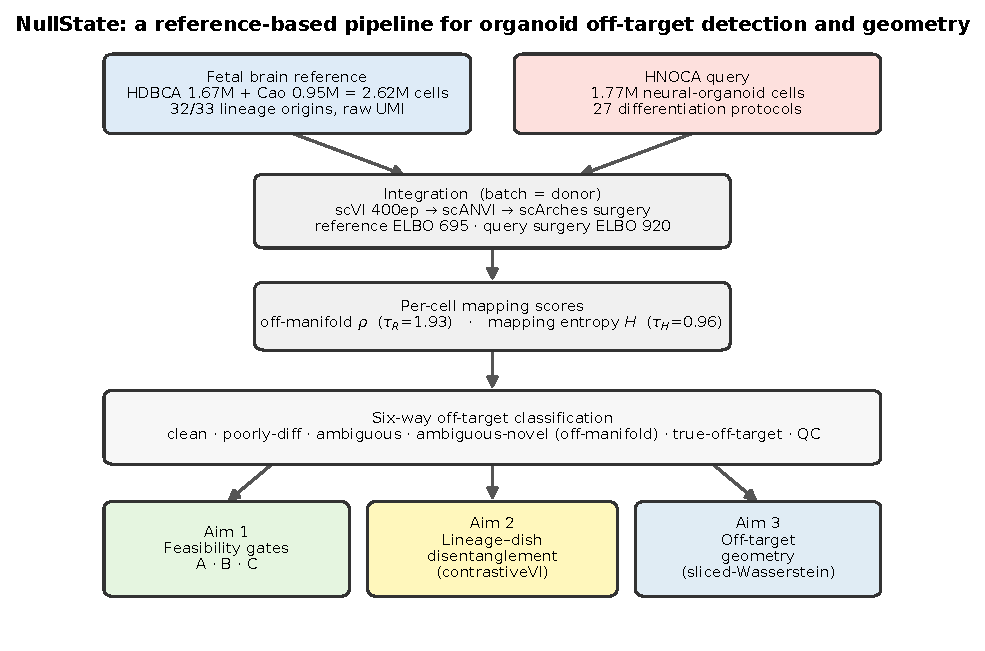
\includegraphics[width=\linewidth]{figs/fig1.pdf}
\caption{\textbf{The NullState pipeline.} A harmonized first-trimester fetal reference (HDBCA $+$
fetal-body atlas; \nref{} cells, raw UMIs) and the HNOCA organoid query (\nquery{} cells, 27 protocols)
are co-embedded by scVI/scANVI followed by scArches reference surgery. Each organoid cell receives two
calibrated mapping scores---off-manifold distance $\rho$ ($\tauR=1.93$) and label entropy $H$
($\tauH=0.96$)---that define a six-state off-target taxonomy, which feeds three analyses: feasibility
gates (Aim~1), lineage--dish disentanglement (Aim~2), and off-target geometry (Aim~3).}
\label{fig:overview}
\end{figure}

\begin{figure}[t]
\centering
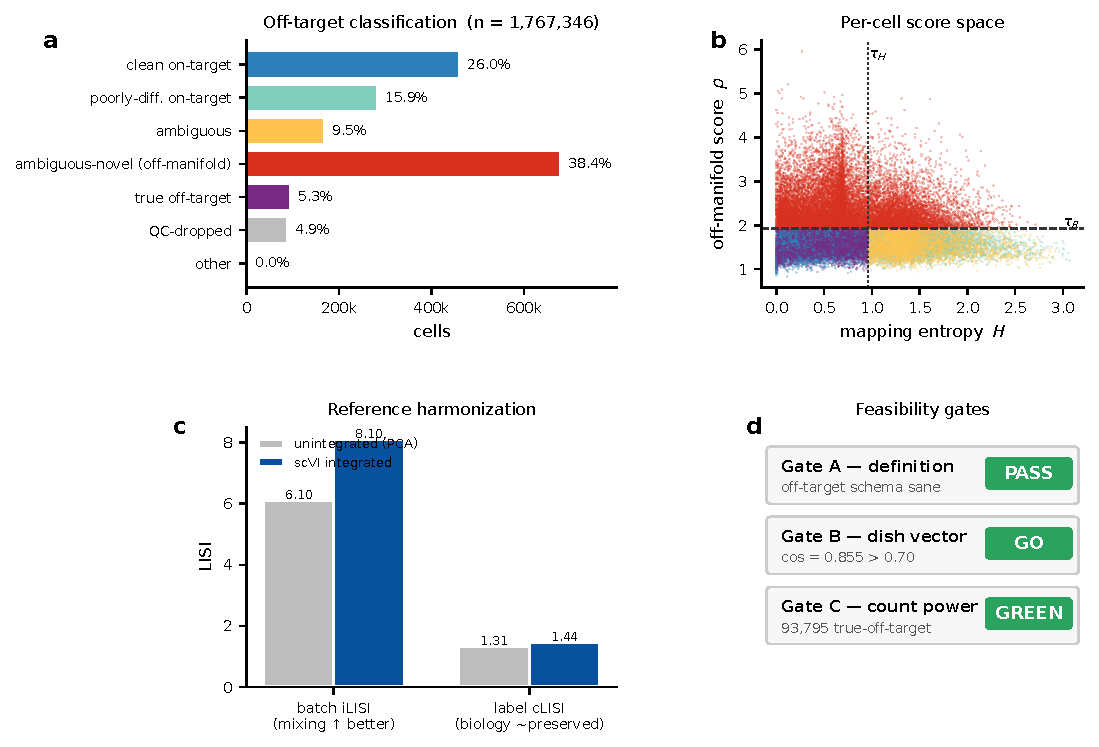
\includegraphics[width=\linewidth]{figs/fig2.pdf}
\caption{\textbf{Harmonized mapping and the off-target landscape (Aim~1).}
(\textbf{a}) Six-state classification of all \nquery{} organoid cells; the off-manifold
\emph{ambiguous-novel} state dominates ($38.4\%$).
(\textbf{b}) Per-cell score space: mapping entropy $H$ versus off-manifold score $\rho$ (subsample),
coloured by class, with the calibrated thresholds \tauH{} (dotted) and \tauR{} (dashed).
(\textbf{c}) Donor-batch integration improves mixing (iLISI $6.10\!\rightarrow\!8.10$) while preserving
biology (cLISI $1.31\!\rightarrow\!1.44$).
(\textbf{d}) The three feasibility gates pass: definition (A), dish-vector self-consistency (B, cosine
$0.855$), and off-target power (C, green).}
\label{fig:aim1}
\end{figure}

\begin{figure}[t]
\centering
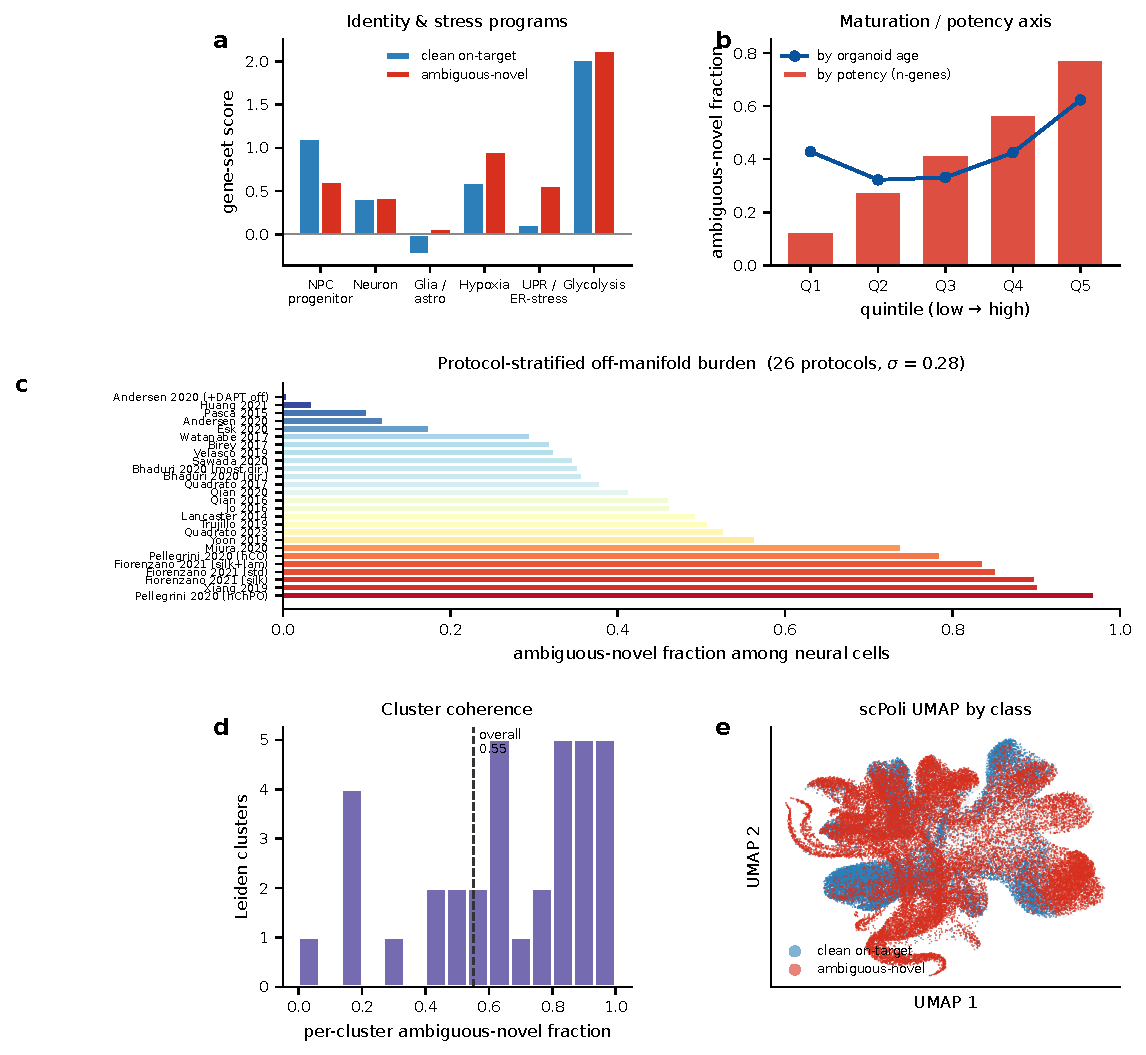
\includegraphics[width=0.92\linewidth]{figs/fig3.pdf}
\caption{\textbf{The off-manifold compartment is structured, not artifactual.}
(\textbf{a}) Ambiguous-novel neural cells lose neural-progenitor identity and gain hypoxia and
unfolded-protein/ER-stress signatures relative to clean on-target neural cells.
(\textbf{b}) Off-manifold fraction increases monotonically with a detected-gene potency proxy (bars)
and with organoid age (line).
(\textbf{c}) Protocol-stratified off-manifold burden spans $0.4\%$--$96.8\%$ across 26 protocols
(colour $=$ fraction); guided cortical protocols are lowest, choroid-plexus/midbrain/thalamic highest.
(\textbf{d}) Per-cluster off-manifold fraction across 30 Leiden communities is bimodal (coherent
populations, not scatter).
(\textbf{e}) scPoli UMAP coloured by class: ambiguous-novel cells occupy contiguous territory.}
\label{fig:diag}
\end{figure}

\begin{figure}[t]
\centering
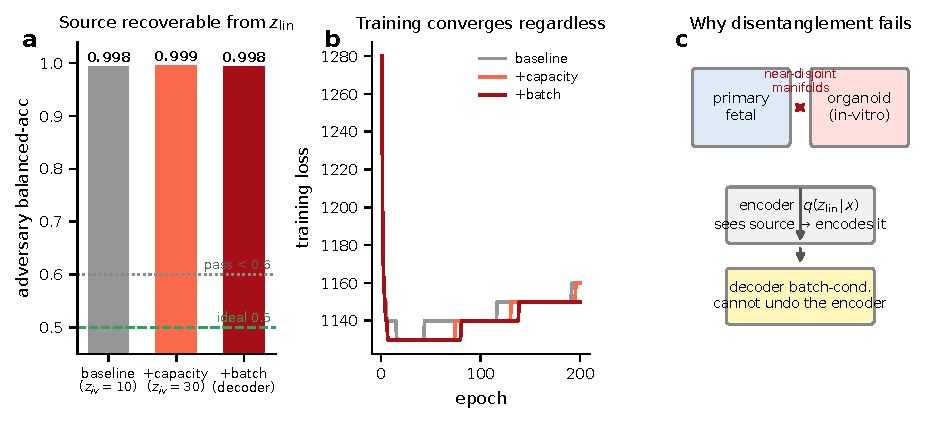
\includegraphics[width=\linewidth]{figs/fig4.pdf}
\caption{\textbf{Lineage--dish disentanglement is not attainable (characterized negative; Aim~2).}
(\textbf{a}) An origin-decoding adversary recovers organoid-versus-primary identity from the
``dish-stripped'' latent \zlin{} at $\geq\!0.998$ balanced accuracy across all interventions (ideal
$0.5$; pass $<0.6$).
(\textbf{b}) Training converges normally in every run, so the failure is structural, not
optimization-related.
(\textbf{c}) Mechanism: near-disjoint primary/organoid manifolds make the background \emph{encoder}
encode source directly; decoder batch-conditioning cannot remove it.}
\label{fig:aim2}
\end{figure}

\begin{figure}[t]
\centering
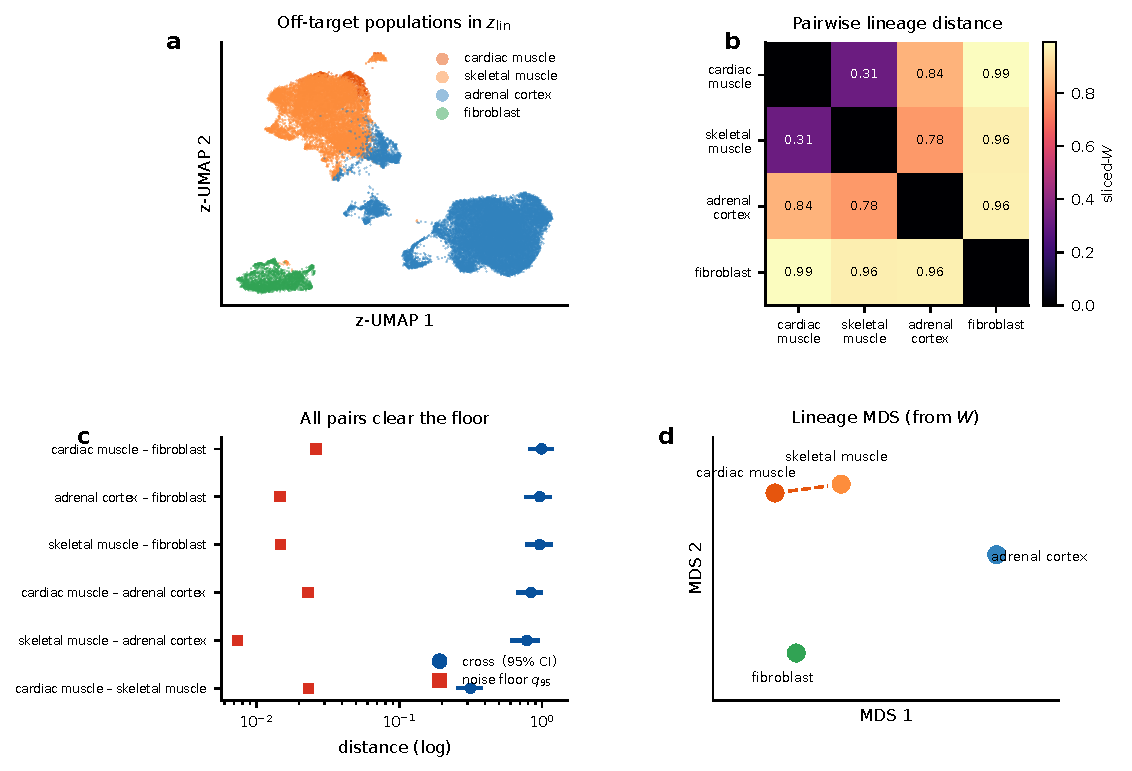
\includegraphics[width=\linewidth]{figs/fig5.pdf}
\caption{\textbf{Off-target geometry is real and biologically ordered (Aim~3).}
(\textbf{a}) Background-latent (\zlin) embedding of the off-target populations; the four well-powered
lineages separate.
(\textbf{b}) Pairwise sliced-Wasserstein lineage-distance matrix.
(\textbf{c}) Every well-powered pair clears its matched-$N$ noise floor ($q_{95}$, red) by
$14$--$105\times$ (cross-distance with $95\%$ CI, blue; log axis).
(\textbf{d}) Multidimensional scaling of the distance matrix: the two myogenic populations (cardiac,
skeletal muscle) are closest, fibroblast most distant, as expected for a lineage embedding.}
\label{fig:aim3}
\end{figure}

% ---------- bibliography ----------
\clearpage
\bibliographystyle{unsrtnat}
\bibliography{refs}

\end{document}
